% Scalar instruction entry source: tools/generate_scalar_instruction_catalog.py.
\subsection{\texttt{ADDTPC}}
\label{sec:scalar-addtpc}
\index{ADDTPC@\texttt{ADDTPC}}
\begin{sloppypar}\noindent\textbf{Purpose.} PC-relative addition (adds to the current PC/TPC).\end{sloppypar}\smallskip
\noindent\textbf{Syntax.}\par
\begin{lstlisting}[style=ptoscalarcode]
addtpc simm, ->RegDst
\end{lstlisting}
\noindent\textbf{Encoding.}\par
\noindent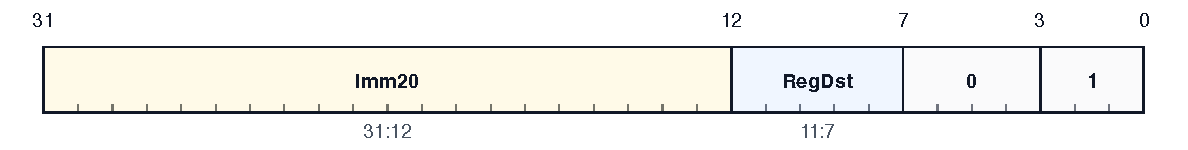
\includegraphics[width=\textwidth]{figs/encoding/scalar_instruction_entries/enc_addtpc.pdf}\par\smallskip
\begin{description}[leftmargin=0.18\linewidth,style=nextline]
\item[Format] \texttt{L32} \texttt{32-bit} scalar word.
\item[Pattern] \texttt{.........................0000111}.
\end{description}
\noindent\textbf{Classification.}\par
\begin{description}[leftmargin=0.18\linewidth,style=nextline]
\item[Category] Branch, Compare, and PC Control.
\item[Family] PC-Relative.
\item[Execution class] \texttt{BRU}; uop\_kind=BRU.
\end{description}
\noindent\textbf{Operand fields.}\par
\begin{description}[leftmargin=0.18\linewidth,style=nextline]
\item[\texttt{RegDst}] Bits \texttt{11:7 (5b)}. 5-bit scalar destination register written by this instruction; X0 is hardwired to zero, so writes to X0 are ignored.
\item[\texttt{imm20}] Bits \texttt{31:12 (20b)}. 20-bit unsigned immediate operand consumed directly by the operation.
\end{description}
\noindent\textbf{Operation.}\par
\begin{lstlisting}[style=ptoscalarcode]
base = CurrentPC()
off = (SignExtend(imm20) << 1)
Write(RegDst, base + off)
\end{lstlisting}
\Needspace{0.08\textheight}
